\documentclass[aspectratio=1610, t]{beamer}  % Frame size = 160mm x 100mm
% \usepackage[utf8]{inputenc}
\usepackage[T1]{fontenc}

\ProvidesPackage{preamble}

% Packages
\usepackage[T1]{fontenc}
\usepackage{fontspec}
\usepackage{xcolor}
% \usepackage{csquotes, soul, graphicx, bbold, subcaption, multirow, mathrsfs, amsmath, listings}
% \usepackage[breaklinks=true,colorlinks=true, linkcolor=blue,urlcolor=blue,citecolor=blue, bookmarks=true,bookmarksopenlevel=2]{hyperref}
% \usepackage[font=footnotesize,labelfont=bf]{caption}
% \usepackage[english]{babel}
% \usepackage{soul, color}
% \usepackage{graphicx}
% \usepackage{wrapfig}
% % \usepackage[font=footnotesize,labelfont=bf]{caption}
% \usepackage{subcaption}
% \usepackage{mathrsfs}
% \usepackage{bbold}
% \usepackage{multirow}
% \usepackage{xcolor}
% % \usepackage[colorlinks,linkcolor=blue,citecolor=blue,urlcolor=blue]{hyper ref}
% \usepackage{lipsum}
% \usepackage{ulem}
% \usepackage{amsmath, amssymb}
% \usepackage{physics}


% Custom commands and settings
\newcommand{\conference}[1]{\gdef\insertconference{#1}}
\newcommand{\authorgroup}[1]{\gdef\insertauthorgroup{#1}}
\setlength{\parskip}{0.5em}  % Space after paragraphs

% References
\usepackage[style=phys, biblabel=brackets, eprint=false, articletitle=false, doi=false, url=false, maxnames=1]{biblatex}
\addbibresource{references.bib}


\title{Sample Title}
\subtitle{Sample Subtitle}
\author[M. Poehlmann]{Michael Poehlmann}
\authorgroup{Offline group}
\institute{UC Davis}
\date{\today}
\conference{DS Offline Meeting}

\usetheme{michael}  % [conference=DS~Offline~Meeting, group=Offline~group]

\begin{document}

\begin{frame}
\titlepage
\end{frame}

\begin{frame}
	\frametitle{First slide example text}
	This is some testy text that explains my point. The text will wrap at some point onto the next line.

	Below is a list with some sample items:

	\begin{itemize}
		\item{item 1}
		\item{Test}
		\item{testy}
	\end{itemize}
\end{frame}

\begin{frame}
	\frametitle{Overview}
	\begin{columns}
		\column{0.45\textwidth}

		This is some text in a column that spans just under half the page width. On the right hand side is an image.

		\column{0.55\textwidth}
		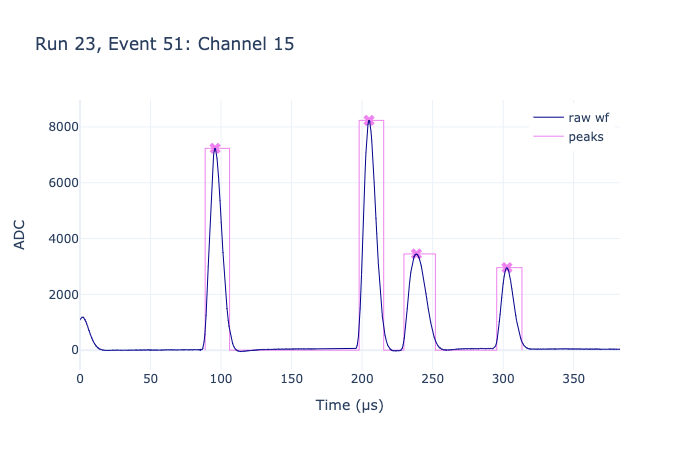
\includegraphics[width=\textwidth]{figs/logo.png}
	\end{columns}
\end{frame}

\begin{frame}{TITLE}
	\begin{block}{Block contain stuff}
		The body of the block. that is pretty long actually look it goes over two lines by now hopefully. The block is used for definitions and whatnot
	\end{block}
	\begin{alertblock}{Alert block}
		OHHH SHIITTT, this must be really important.
	\end{alertblock}
	\begin{exampleblock}{Example block}
		An example of something awesome.
	\end{exampleblock}
\end{frame}

\end{document}